\chapter{Introduction}
\label{introduction}
Modern physics tells that there are four fundamental forces which can describe all observable the Universe. There are gravitational, electromagnetic, strong and weak interactions. Three of them are combined to the Standard Model, except the gravitational one. A scale comparable to a size of no more than the size of atomic nuclei is a field studied within the nuclear physics in close connection with the particle physics.

Nuclear physics studies the properties and structure of atomic nuclei and their reactions. Some of its main tasks are related to the analysis of the nature of nuclear forces acting between nucleons (protons and neutrons) that form nuclei and to identify and explain the properties of their motion. Understanding nuclear forces is fundamental for both theoretical and experimental nuclear physics as well as for applied nuclear physics, in particular for nuclear medicine. Currently, it is known that nuclear interaction between nucleons is a residual interaction of the strong interaction between even finer elements of matter --- quarks and gluons and which is described by the Quantum Chromodynamics (QCD). As is well known, nowadays we are not able to solve QCD in the non-perturbative region (at the low-energy scale) and thus to describe processes at nuclear scale starting from quarks and gluons and their interactions. For the first ongoing attempts in lattice QCD, see e.g. Refs.~\cite{Beane2011, Aoki2011}. For example, the obtained deuteron binding energy is still much larger than the experimental value~\cite{Beane2013, orginos2015two}. %, but after a couple of years the authors managed to get closer to the expected value, but with a pion mass of $m_{\pi}$ $\sim$ 450 MeV~\cite{orginos2015two}.
Another advanced approaches, like the Lattice Effective Field Theory~\cite{Li2018}, also fail to deliver results of quality comparable with the standard nuclear physics techniques. By the latter ones we understand approaches based on the effective nuclear interactions defined as interactions among nucleons and relying mainly on meson exchange processes. 
%The interesting reader would find in~\cite{machleidt2011chiral, Machleidt2014, Soma2018} as guidelines to study fully the main developments in nuclear structure theory from a historical perspective starting the discovery of the neutron and to date.

As a result, effective and phenomenological models of nuclear interactions are still of great importance in low-energy nuclear physics~\footnote{In my doctoral research, done as part of the investigations within the Krak{\'o}w's group, low-energy nuclear physics is understood as nuclear physics at energies below the pion production threshold.} and various \textit{ab initio} techniques to obtain predictions have been derived. Calculations within the \textit{ab initio} or \textit{microscopic} techniques mean that the nuclear $A$-few body problem can be formulated in terms of the nonrelativistic Schr\"odinger equation using various NN local or non-local interactions with or without the inclusion of many-body forces. Independently on the problem in hand: the bound state of nucleons, nuclear reactions, production or decay processes, the starting point of research is a construction of the complete Hamiltonian of the system of interacting particles. This thesis is devoted to purely nucleonic processes, in particular, to three-nucleon processes: the elastic and inelastic neutron-deuteron scattering. 

The general form of the nuclear Hamiltonian for the system \textit {A} of nucleons is
\begin{equation}
H = \sum\limits_{i = 1}^{A}\frac{p^{2}_{i}}{2m_{i}} + \sum\limits_{i,j}^{A}V_{ij}^{\mathrm{2N}}+ \sum\limits_{i,j}^{A}V_{ijk}^{\mathrm{3N}} + \ldots + V^{A\mathrm{N}}\;,
\label{Eq21}
\end{equation} 
where the first term is the non-relativistic kinetic energy, $m_{i}$ and $p_{i}$ are the $i$-th nucleon mass and momentum, respectively, and $V^{\mathrm{2N}}_{ij}$, $V^{\mathrm{3N}}_{ijk}$ and $V^{A\mathrm{N}}$ represent the two-, three and $A$-nucleon potentials, respectively. 
The definition~(\ref{Eq21}) is used e.g. for a bound state $\ket{\Psi_{A}}$ in the time-independent Schr\"odinger equation formulated as an eigenvalue problem $\ket{\Psi_{\mathrm{bound}}}$
\begin{equation}
H\ket{\Psi_{A}} = E\ket{\Psi_{A}}\;,
\label{Eq22}
\end{equation}
where $E$ is the binding energy. 
%In general, this equation can be considered in coordinate or momentum space. In addition, working with the isospin concept of nucleons, this equation reduces to partial wave decomposition (PWD), see Chapter~\ref{formalism}.

There are a few mathematical algorithms and \textit{ab initio} approaches with well-controlled approximations for solving a $A$-nucleon Schr\"odinger equation for light nuclei. In general, this equation can be considered in coordinate or momentum space. Some examples of \textit{ab initio} methods for calculations of few-nucleon systems with $A \geq$ 4 were listed and reported in an overview~\cite{leidemann2013modern}. For example, one of these methods is approach basing on the Faddeev-Yakubovsky equation, which was used to calculate the binding energy and the wave function of $^{4}$He~\cite{nogga2000modern}. I would like also to mention methods which are quite precise in describing the properties of light and medium mass nuclei up to $A$ = 12, i.e. methods based on Monte Carlo algorithms, such as the Monte Carlo variational (VMC) or the Monte Carlo with Green's function (GFMC) methods, see Ref.~\cite{carlson2015quantum}. It is also worth mentioning that there are methods associated with the shell model of nuclei, as the no-core shell model (NCSM)~\cite{navratil2016unified}, the No-Core Configuration Interaction (NCCI)~\cite{maris2015emergence} model, or the realistic shell model (RSM)~\cite{fukui2018realistic}. In the last decade, many efforts have been made to use the Similarity Renormalization Group (SRG) approach with a combination of the chiral interaction, see e.g. Ref.~\cite{epelbaum2019few}. The SRG approach is based on the unitary transformation of the many-body Hamiltonian system to decouple states with high and low momenta~\cite{bogner2010low, hergert2016medium}. Such transformed Hamiltonian can be next used in the above-mentioned computational schemes.
In the case of $A \leq$ 4 nuclear bound systems, the hyperspherical harmonic (HH) method has been developed and applied by the Pisa group~\cite{kievsky2008high}.

The latter method can also be applied to describe the elastic Nd scattering at the very low ($\leq 10$ MeV) incoming nucleon laboratory energies, working in coordinate or in momentum space~\cite{marcucci2009n, marcucci2019hyperspherical}. However, to study 3N scattering a few \textit{ab initio} approaches based on the Faddeev equations scheme~\cite{faddeev2016scattering} are currently the most effective tool. The Krak{\'o}w-Bochum group developed the Faddeev formalism for rigorous calculations applied to 3N continuum observables, see Ref.~\cite{Glockle1996} for a general overview. Interesting computational technique based on the 3N continuum Faddeev calculations with lattice-like discretization in momentum space was developed in~\cite{rubtsova2012three}. In 3N systems as well as beyond them, the Faddeev formalism can be realized in a couple of ways, like the Alt-Grassberger-Sandhas (AGS) equations~\cite{fonseca2017numerical} with the possibility to include the Coulomb interaction between protons~\cite{deltuva2019coulomb} and the Faddeev-Yakubovsky for five-nucleon calculations~\cite{lazauskas2018solution}.  
%The interesting reader can find another good overview of state-of-the-art ab initio calculations of the bound state and scattering observables in Ref.~{johnson2019bound} and references therein. 
Another recent overview of state-of-the-art \textit{ab initio} calculations of the bound state and scattering observables is given in Ref.~\cite{johnson2019bound} and references therein.

The deuteron is the only one stable bound state of two nucleons~\footnote{It should also be noted that there is a state consisting of two bound protons (di-proton)~\cite{Raciti2008}, which can be considered as the isotope $^{2}$He of helium but its lifetime is very short. As for the two bound neutrons (di-neutron), at the moment there is no experimental evidence of its existence.}. Analyzing its properties, it was found that nuclear forces of short-range nature with a range of not more than 2 $\divisionsymbol$ 3 fm. The experimental data on the nuclei and nuclear reactions, including a huge amount of data on nucleon-nucleon (proton-proton and proton-neutron) scattering, led to the conclusion that nuclear forces can be considered in the first approximation as a two-particle interaction. Thus, the problem of describing nuclear interactions can be approximately formulated as a problem of determining the two-nucleon (2N) potential $V^{\mathrm{2N}}$. %for the entire nucleus instead of considering all its nucleon components.

In general, no matter what strategy (phenomenology, meson exchange picture, etc.) is chosen to build a model of nuclear interactions, the properties of nuclei are taken into account. With increasing number of nucleons, the volume of nuclei increases proportional to the mass number ($A$ > 4), what is explained by the fact that the central nuclear force is a short-range force and strongly attractive at this range. This is a saturation effect. The nuclear force depends not only on the range between nucleons (central force), but also on the mutual orientation of spins (spin-spin force), the mutual direction of the spin and the orbital angular momentum (spin-orbital force), and also on the orientation of the spins of each nucleon to the relative distance between them (tensor force). The existence of a spin-orbit force helps to explain the experimentally observed magic numbers for nucleons. Specifically, the presence of a quadrupole moment in the deuteron is result of a tensor force contribution. It is also often convenient to split the nuclear force to a sum of two (short- and long-range) or three (short-, intermediate- and long-range) terms. 

The first non-trivial model of nuclear force was the NN potential developed by Hideki Yukawa~\cite{yukawa1935interaction}. Yukawa used the idea that the nucleons interact via exchanges of unknown particle, and combined it with the idea of the short-range interaction. He predicted that this particle should obey the Einstein-Bose statistics and estimated its mass. Today, we identify this particle as the $\pi^{0}$-meson pseudoscalar boson (with total spin 0 and odd parity). Further development of nuclear forces show by the end of the 60s that the NN interaction includes not only a one-pion interaction but also with two pion processes, and much heavier mesons exchanges depending on the inter-nucleon distance. In the 90s, the most known and frequently used the meson-exchange NN models were the Paris potential~\cite{cottingham1973nucleon}, the Bonn potential~\cite{machleidt1987bonn}, and two potentials provided by the Nijmegen group --- the non-local Nijmegen potential (Nijm I) and its the local version (Nijm II)~\cite{stoks1993partial}. During works on their potential, the Nijmegen group collected 1787 $pp$ data and 2514 $np$ data and applied a 3$\sigma$-rejection criterion and other statistical methods to make the database self-consistent. They performed partial-wave analysis (PWA93) below 350 MeV and the Nijmegen database (or the 1992-database) was obtained. Due to this, they were able to describe 2N scattering data using their potentials with $\chi^{2}/\textrm{datum}\approx$~1.08.
%in describing 2N data. 
%In addition, in 1993 a group in Nijmegen had published a new partial wave analysis (PWA) of all nucleon-nucleon scattering data below 350 MeV and they managed to reach the magnitude of $\chi^{2}/\textrm{datum}\approx$~1.08 obtained from a comparison of theoretical predictions and experimental data. 
%Then PWA will later be used for optimizing and testing so-called \textit{realistic} NN potentials. 
All above-mentioned models combine a meson exchange theory with a phenomenological approach in the derivation of NN potentials which base upon the operator structure. In general, such a phenomenological NN potential consists of linear combinations of terms which are deduced from the nuclear properties and symmetries. An interested reader can find more detailed information on how the theory of nuclear structure has developed from a historical perspective, from the discovery of the neutron to the present day, as well as a review of NN interactions in Refs.~\cite{Machleidt2014, naghdi2014nucleon, zhaba2017deuteron, machleidt2017historical, Soma2018}.
%At the beginning of the 21st  century, only a few models of the NN interaction provided an accurate description of 2N sector data. At that time the most successful models were the mentioned Nijmegen (I, II), the Argonne V18 (AV18)~\cite{Wiringa1995} and the CDBonn~\cite{Machleidt2001} potentials which very accurately described the properties of a two-nucleon (2N) bound and scattering systems. In the case of the AV18 the long-range part of the interaction, given by the one-pion-exchange, was supplemented by a purely phenomenological short-range part, for the CD-Bonn model also the short-range part was described via exchanges of heavier mesons and processes with multiple meson exchanges. Both forces achieved mentioned-above $\chi^{2}$/datum magnitude close to 1 but using nearly 50 free parameters. These parameters were fitted, via the phase shifts obtained by the Nijmegen group~\cite{stoks1993partial}, to all NN data available at that time. In addition, the CD-Bonn potential had taken into account the latest set of experimental NN data as accurately as possible at that time. In both cases, only the central values of the parameters were determined and no information about their uncertainties, to the best of our knowledge, was published. In the course of time, the expectations of the improvement in the accuracy of the fitting procedure grew. The new, usually very precise data, were taken into account~\cite{Machleidt1996}. The important step was taken by Rodrigo Navarro P{\'{e}}rez and his collaborators from the Granada group, who carefully revised the whole nucleon-nucleon database. They prepared a new database~\cite{Perez2013}, removing from the previously used data set, experimental results for which the experimental uncertainties had been unknown or poorly defined. They excluded also datasets inconsistent with other data, what led to self-consistency of the eventually accepted data sets. The extended statistical tests of this database, presented in~\cite{Perez2013} confirmed the internal consistency of the data kept in this database. This database is currently a standard set of data used for fixing parameters of the NN forces. For us, the most important examples of such models are the One-Pion-Exchange-Gaussian (OPE-Gaussian) force derived by the Granada group~\cite{NavarroPerez2014}, other forces from the same group~\cite{Perez2015} and the newest chiral interactions from the Bochum-Bonn group~\cite{Reinert2018}. The models from Refs.~\cite{NavarroPerez2014} and~\cite{Reinert2018} which were applied in this work are described in Section~\ref{potentials} of Chapter~\ref{formalism} in detail.

At the beginning of the 21st  century, the most successful \textit{realistic} models of the NN force were the above-mentioned Nijmegen (I, II), the Argonne V18 (AV18)~\cite{Wiringa1995} and the CD-Bonn~\cite{Machleidt2001} potentials which provided an accurate description of the 2N scattering data and deuteron properties. In the case of the AV18 the long-range part of the interaction, given by the one-pion-exchange (OPE), was supplemented by a purely phenomenological short-range part. For the CD-Bonn model the short-range part was described via exchanges of heavier mesons and processes with multiple meson exchanges. The AV18 and the CD-Bonn potentials have 40 and 43 potential force parameters, respectively. The AV18 potential parameters were fitted using the above-mentioned Nijmegen PWA93 results. Before the year 2000, the new sets of experimental 2N data were collected and together with the 1992-database built the 1999-database~\cite{Machleidt2001}. The resulting 1999-database was taken into account to construct the CD-Bonn potential. The quality of description can be quantified by the magnitude of $\chi^{2}$/datum obtained from a comparison of theoretical predictions and experimental data. In the case of the AV18 potential $\chi^{2}$/PWA92 = 1.09 and $\chi^{2}$/PWA99 = 1.21. 
For the CD-Bonn model $\chi^{2}$/datum = 1.02 for both databases~\cite{Machleidt2001}. For the both potentials, only the central values of the parameters were determined and no information about their uncertainties, to the best of our knowledge, was published. In the course of time, the expectations of the improvement in the accuracy of the fitting as well as in establishing parameter uncertainties procedure grew. 

The important step in establishing the 2N potential parameters was taken by Rodrigo Navarro P{\'{e}}rez and his collaborators from the Granada group, who carefully revised the whole 2N database. They prepared a new database (Granada-2013 database)~\cite{Perez2013}, removing from the previously used data, those for which the experimental uncertainties had been unknown or unclear defined. They excluded also data sets inconsistent with other data, which led to the self-consistency of the eventually accepted data. The procedure is described in Chapter~\ref{OPEG-potential} in more detail.
The extended statistical tests of this database presented in~\cite{Perez2013} confirmed the internal consistency of the accepted data. The Granada-2013 database is currently a standard set of data used for fixing parameters of the NN forces what can be done by fitting parameters to the extracted phase shifts or to 2N data directly. The free parameters of the both models of the NN force used in this thesis: the OPE-Gaussian~\cite{NavarroPerez2014} and the family of the chiral SMS interactions from the Bochum group~\cite{Reinert2018} have been fixed with the Granada-2013 database. Specifically the OPE-Gaussian potential has been derived already by R. Navarro P{\'{e}}rez from Granada. This potential is discussed in Chapter~\ref{OPEG-potential} in detail.

%For my research program, the most important examples of such models are the OPE-Gaussian potential derived by the Granada group~\cite{NavarroPerez2014} and the family of chiral SMS interactions from the Bochum group~\cite{Reinert2018}.

Currently, the most sophisticated models of nuclear forces at the low-energy regime are chiral interactions. S. Weinberg was the first who proved, in his seminal papers~\cite{weinberg1990nuclear, weinberg1991effective}, that it is possible to build Lagrangian for all possible interactions between pions and nucleons in agreement with the symmetries (including the broken chiral symmetry) and properties of low-energy QCD, and to construct effective Hamiltonian in terms of nucleons and pions. In this construction an infinite number of terms corresponding to the Feynman diagrams for the Lagrangian can be rewritten as an pertubative expansion with respect to some parameter. Each term in this Lagrangian is multiplied by the corresponding coupling constants, the so-called low-energy constants (LECs), which needs to be determined from experimental data in nucleonic or $\pi$-N sector~\cite{Reinert2018, epelbaum2019high}. The power counting scheme allows to organize a perturbative ordering of the Lagrangian terms and thus point terms dominant in the potential. The expansion parameter depends on the ratio between the low- and high-energy scales. It is assumed to have the form $Q = \mathrm{max}\left(\frac{p}{\Lambda_{\chi}},\frac{m_{\pi}}{\Lambda_{\chi}}\right)$, where $\Lambda_{\chi}$ is the chiral symmetry breaking scale, whose value is a priori set of the order of $\rho$-meson mass ($\Lambda_{\chi} = 770$ MeV), however, values in range 600~MeV~\cite{Epelbaum2015} -- 1~GeV~\cite{Entem2017} are used~\cite{Reinert2018},~\cite{Furnstahl2015},~\cite{epelbaum2020towards}.
Further $p \equiv |\vec{p}|$ is the magnitude of the external (nucleon) three-momenta in the center of mass scattering system (c.m.s), and $m_{\pi}$ is the pion mass. Important feature of the chiral expansion in powers $\nu$ of $\left(Q/\Lambda_{\chi}\right)$ is a finite number of diagrams at a given order which make theory computable. Finally, an effective potential can be derived from the effective Lagrangian with e.g. the method of unitary transformations~\cite{epelbaum2010nuclear, epelbaum2019high}. This leads to nuclear forces emerging as a hierarchy controlled by the $\nu$, see Figure~\ref{hierarchy}, and gives a nice explanation of various stength of contributions to two- and many-body forces obtained within the Chiral Effective Field Theory ($\chi$EFT). 
In general, the expansion of the NN force has the form
\begin{equation}
V_{\mathrm{2N}} = V^{(0)}_{\mathrm{2N}} + V^{(2)}_{\mathrm{2N}} + V^{(3)}_{\mathrm{2N}} + V^{(4)}_{\mathrm{2N}} + V^{(5)}_{\mathrm{2N}} + \ldots\;,
\end{equation}
with the superscripts referring to the power $\nu$ of the expansion parameter $(Q/\Lambda_{\chi})^{\nu}$.
For example, in the lowest leading order ($\nu$ = 0) the NN potential is made up by two terms, represented by the graphs in the first row of Figure~\ref{hierarchy}. They are the static one-pion exchange ($V_{1\pi}$) and the contact interaction ($V_{\mathrm{cont}}$) between two nucleons. The latter plays the role of a short-range interaction. For $\nu$ = 1 all terms cancel and give no contribution to the NN interaction. At the higher orders of the chiral expansion more terms containing multiple mesons exchanges and various types of contact terms occur.
At the next-to-next-to-leading order (N$^{2}$LO), which corresponds to $\nu$ = 3, the NN potential involves contributions from the one-, two-exchange and contact terms with up to three derivatives which enters new short-range interactions contributing at this order. In addition, for a 3N system a 3N force appears, for the first time, at this chiral order.
\begin{figure}[h]
\begin{center}
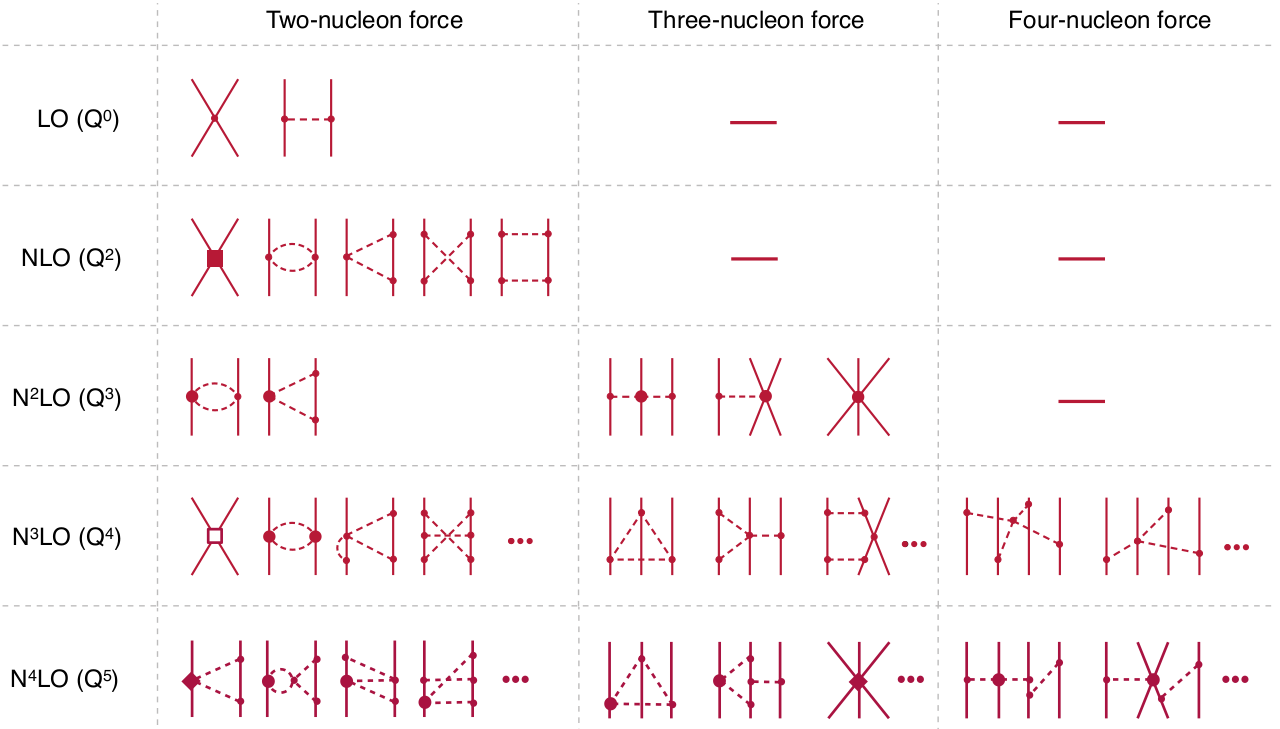
\includegraphics[width=1\textwidth]{PhD-text/3_Potentials/chi_expan_nf_EE.png}
\end{center}
\caption{Hierarchy of nuclear forces in $\chi$EET at increasing orders in chiral expansion based on the Weinberg scheme. Figure is taken from Ref.~\cite{epelbaum2019high}. Solid and dashed lines represent nucleons and pions, respectively. Solid dots, filled circles, filled squares, filled diamonds, and open squares denote vertexes arising at corresponding order $\nu_{i}$ ($i = 0, 2, 3, 4, 5$) of the effective Lagrangian, respectively. (Image source: \url{https://www.frontiersin.org/files/Articles/515888/fphy-08-00098-HTML/image_m/fphy-08-00098-g002.jpg}; use permitted under the Creative Commons Attribution License CC BY 4.0.)}
\label{hierarchy}
\end{figure}
%Therefore to reduce numerous Feynman graphs and make theory calculable one have to make a  perturbative expansion in powers of $(Q/\Lambda_{\chi})^{\nu}$, where the power $\nu$ is a power counting, which is defined by~\cite{epelbaum2019high}
%\begin{equation}
%\nu = -2 + \sum_{i}V_{i}\kappa_{i}
%\end{equation}
%where $V_{i}$ is the number of vertices of each contribution and $\kappa_{i}$ is the inverse mass dimension of the corresponding LEC, which it turns out,  the number of derivatives or pion-mass insertions and ni the number of nucleon fields (nucleon legs) involved in vertex i
%\footnote{but a priori is should be estimated to be of order of}

Nowadays, there are few groups engaged in derivation of chiral forces and two of them have dominated the field: the Bochum-Bonn group (see Refs.~\cite{Epelbaum2015,Epelbaum2006,Epelbaum2009,Epelbaum2015a} and more recently~\cite{Reinert2018}) and the Moscow(Idaho)-Salamanca group (see Refs.~\cite{Entem2017,Machleidt2011,Machleidt2013,Machleidt2016,Machleidt2018}). Both teams start from the same Lagrangian but due to various methods used, their final potentials differ. 

The important difference between their approaches is using various ways of regularization of the chiral nuclear potential. In particular, the Moscow(Idaho)-Salamanca collaboration uses a non-local regularization procedure in momentum-space for both the long- and short-range contributions~\cite{Entem2017}. The regulator function of the initial $p$ and final $p^{\prime}$ relative momentum of two nucleons is taken as 
\begin{equation}
f (p^{\prime}, p) = \mathrm{exp}\left[-\left(\frac{p^{\prime}}{\Lambda}\right)^{2n} - \left(\frac{p}{\Lambda}\right)^{2n}\right]\;,
\end{equation}
where $n$ depends on the chiral operators (e.g., $n =$~4 for the one-pion exchange potential). The three values of the cutoff parameter $\Lambda =$~450, 500, and 550 MeV were used while fitting potential parameters which resulted in three versions of this potential~\cite{Entem2017}.
%for this potential and are also used in~\cite{Entem2017}. 
%The three values were used while fitting potential parameters resulting in three versions of this potential.
Obtained $\chi^{2}$/datum values depend on the regularization parameter $\Lambda$, the order of chiral expansion, the energy range, and the isospin channel. In the case of the next-to-next-to-next-to-next-to-leading order (N$^{4}$LO) potential and $\Lambda$ = 500 MeV, $\chi^{2}$/datum = 1.15 for the fit of the 2016-database~\footnote{2016 database bases on the 1999 database and consists of 2932 pp and 3058 np data and including the data published between 2000 and 2016 which are not discarded by the Nijmegen criteria~\cite{Bergervoet1988}. 
%The authors of Ref.~\cite{Entem2017} are aware about the Granada-2013 database constructed on applying the modified rejection criteria from Ref.~\cite{Gross2008}, but they wants to be consistent with the 1999 database for which the Nijmegen criteria have been applied. In turn, the 1999 database is build of 1992 database of 1787 pp data in Ref.~\cite{Bergervoet1990} and 2514 np data in Ref.~\cite{Stoks1993} and supplemented by 1145 pp and 544 np data (given in Tables XV and XVI of Ref.~\cite{Machleidt2001}, respectively), which were collected up to 1999 and then the Nijmegen rejection criteria were applied by R. Machleidt in Ref.~\cite{Machleidt2001}.
} (see~\cite{Entem2017} for details) of combined $np$ and $pp$ data in the energy range 0–290 MeV. 

In their first works, the Bochum-Bonn group also proposed and used a non-local regulator. However, due to observed strong artefacts the newest models of the Bochum-Bonn group, use the semilocal~\footnote{The term ``semilocal" means which the nuclear force is regularized locally for the long-range part and non-locally for the short-range one.} regularization. It can be applied either in  coordinate space with the regulator function,
\begin{equation}
f(r) = \left[ 1- exp\left(-\frac{r^{2}}{R^{2}}\right)\right]^{6}\;,
\label{reg_coord}
\end{equation}
where $r$ is the internucleon distance and $R$ is the regulator parameter,~\cite{Epelbaum2015, Epelbaum2015a}; or in momentum space by changing the meson propagator, see Ref.~\cite{Reinert2018}. 

%In momentum space can be regulated with the non-local Gaussian regulator
%%The regulator function
%%In the latter case, the contact interaction $V^{(i)}_{cont}$ can be regulated in momentum space with the  nonlocal Gaussian regulator
%\begin{equation}
%f (p^{\prime}, p) \propto exp\left(-\frac{(m^{2}_{\pi} - q^{2})}{\Lambda^{2}} \right)\;,
%\end{equation}
%where $q \equiv \mid\vec{p}^{~\prime} - \vec{p} \mid$, $\vec{p},~\vec{p}^{~\prime}$ are the initial and final relative momenta of nucleons and $\Lambda$ is an ultraviolet cutoff whose values lie in the range of $\Lambda$ $\in \left[350, \ldots, 550\right]$ MeV, see Ref.~\cite{Reinert2018}.
%To achieve the assigned goals outlined briefly in the Overview 
In this thesis I use the chiral NN potentials up to N$^{4}$LO$^{+}$ order (the N$^{4}$LO potential supplemented by some terms from the sixth order N$^{5}$LO force) with regularization applied in momentum space (the SMS forces). This force is described in Chapter~\ref{chiral_model} in detail.

The understanding of nuclear systems is limited if using only NN potentials beyond 2N systems. In principle, the NN potentials can well describe 3N systems, and most of the results are in good agreement with the available experimental data at laboratory nucleon scattering energies of up to 100 MeV~\cite{Glockle1996}. However, there are some large discrepancies between theory and experiment already in the 3N system, for example, the triton binding energy problem~\cite{nogga1997triton, nogga2003three, perez2014triton}, the $A_y$-puzzle (the problem of describing the nucleon analyzing power for the elastic Nd scattering up to 30 MeV)~\cite{entem2002chiral}, and the description of the deuteron breakup cross section for the symmetric space star (SST)
and quasi-free scattering (QFS) configurations~\cite{witala2010discrepancies, witala2011nn}. Therefore, in order to obtain a more accurate description of 3N system, a NN interaction must be supplemented by a 3N force acting in this system.

Among all of the many-nucleon forces, the 3N force is the most intensively studied, but its structure is still unclear. Currently, the important models of 3NF are the semi-phenomenological ones: the Tucson-Melbourne~\cite{coon1979two, coon1981two, coon2001reworking} force, the UrbanaIX~\cite{pudliner1997quantum} potential and models arising from $\chi$EFT. The latter have been derived mainly by the Bochum-Bonn group, starting from the seminal paper~\cite{epelbaum2001three} where the 3NF effects in the nucleon-deuteron scattering up to the next-to-next-the leading order (N$^{2}$LO) were investigated. The 3N interaction, similarly to the two-nucleon one is derived within the chiral approach in a perturbative way~\cite{Epelbaum2009, Machleidt2011}. It occurs for the first time at the N$^{2}$LO and has at this order only two free parameters, (the low-energy constants commonly denoted $c_{D}$ and $c_{E}$). Already in the work~\cite{epelbaum2001three} the problem of fixing of these parameters had to be addressed. The authors chose the $^{3}$H binding energy and the nucleon-deuteron doublet scattering length $^{2}$a$_{\textrm{nd}}$  to find $c_{D}$ and $c_{E}$ values. The same procedure to fix $c_{D}$ and $c_{E}$ was also used at the next (N$^{3}$LO) order of chiral expansion with new diagrams for 3NF taken into account~\cite{skibinski2011triton}. These new contributions to the 3NF do not introduce new free parameters, however at the next (N$^{4}$LO) order again several free parameters are expected~\cite{girlanda2011subleading}. Another strategy of fixing 3NF's parameters was used recently for the next generation of the chiral models --- with semilocal regularization in coordinate space~\cite{epelbaum2019few}. At the moment the 3NF with regularization in coordinate space is available only up to N$^{2}$LO and this dominant 3NF contribution is used in~\cite{epelbaum2019few}. Here, beside the $^{3}$H binding energy, the total and differential cross sections at $E =$ 70 MeV and at $E$ = 108 MeV around its minimum were used to fix the $c_{D}$ and $c_{E}$ parameters. The use of the cross section instead of the nucleon-deuteron doublet scattering length was imposed by the strong correlation between the $^{3}$H binding energy and the nucleon-deuteron doublet scattering length (the so-called Phillips line)~\cite{phillips1968consistency}, which could bias the fitting procedure and lead to incorrect $c_{D}$ and $c_{E}$ values. The choice of the cross section as the new observable was dictated by the fact that big 3NF effects are observed for this observable above $E\approx$ 60 MeV, thus a sensitivity of theoretical predictions to the values of free parameters had been expected. Another reason for using the cross section was the existence of the very precise experimental data~\cite{sekiguchi}. Nevertheless, the values of $c_{D}$ and $c_{E}$ obtained in~\cite{epelbaum2019few} suffer from relatively large uncertainties and are (for the regulator parameter $R$ = 0.9 fm): $c_{D}$ = 2.1 $\pm$ 0.9 and $c_{E}$ = -0.329 (+0.103, -0.106), so the uncertainty amounts up to 30\%-40\%, being quite substantial. The magnitudes of the free parameters and their uncertainties depend also on the value of the regulator parameter and for $R$ = 1 fm one finds $c_{D}$ = 7.2 $\pm$ 0.9 and $c_{E}$ = -0.381 (+0.117, -0.122), so the uncertainty here reaches 12\%-30\%. Such big values of parameters' uncertainties suggest that usefulness of other observables to fix 3NF free parameters is worth investigating as it can lead to a more precise determination of the $c_{D}$ and $c_{E}$ values. 
%Of course the data description is excellent in both cases. Both models are described in details in Chapter~\ref{potentials}

Investigation of Nd scattering within the Faddeev equations in momentum space is a good tool to study not only NN potential but also 3N force. A comprehensive overview of 3N calculations with various semi-phenomenological NN potentials is given in Ref.~\cite{Witaa2001}. Similar works were recently conducted as part of the LENPIC (Low-Energy Nuclear Physics International Collaboration project) by applying the chiral interaction ~\cite{binder2016few, binder2018few, epelbaum2019few} with the coordinate space semilocal regularization (the SCS potential)~\cite{Epelbaum2015} and with the momentum space semilocal regularization (the SMS potential)~\cite{Reinert2018, epelbaum2020towards}. 

During the last ten years, in parallel to the development of the nuclear force models, the question how to estimate the uncertainties of predictions is also being considered. For example, various ideas for estimating theoretical uncertainties have been proposed and discussed within the $\chi$EFT framework, see Refs.~\cite{melendez2017bayesian, Epelbaum2015, Furnstahl2015, ekstrom2013optimized, perez2015low}. In Ref.~\cite{Epelbaum2009} a simple approach for estimating the theoretical uncertainty in few-nucleon calculations by the cutoff dependence was suggested. However, as was shown by E. Epelbaum, H. Krebs, and Ulf-G. Mei{\ss}ner (EKM)~\cite{Epelbaum2015}, such procedure has some disadvantages, namely does not allow one to evaluate precisely the effects of neglected interactions. Therefore in~\cite{Epelbaum2015}, they proposed and applied for 2N observables new method (``EKM prescription") for estimating truncation errors, which are uncertainties arising from neglecting higher orders of the chiral expansion for the 2N potential. This algorithm was adopted also for many-nucleons systems, in the cases where predictions are based on a NN interaction~\cite{binder2016few,binder2018few} only orr on NN+3N force~\cite{epelbaum2019few}. However, since the EKM prescription does not provide a statistical interpretation of truncation errors, a Bayesian approach for calculating the posterior probability distribution for predictions in the chiral EFT was developed, see Refs.~\cite{melendez2017bayesian, Furnstahl2015} focused only on 2N observables. 

As mentioned above, there is one more additional source of theoretical errors ---\\ the statistical errors arising from the propagation of uncertainties of free parameters of a NN interaction. For the first time, it was studied with the OPE-Gaussian potential in the description of the elastic Nd observables~\cite{Skibinski2018}. In recent paper~\cite{volkotrub2020uncertainty} we investigated the magnitudes of statistical uncertainties of 3N observables of the elastic and inelastic Nd scattering at energies up to 200 MeV predicted by the chiral SMS potential at different orders of chiral expansion up to N$^{4}$LO$^{+}$. Last but not least, there are the uncertainties arising from using the various models of nuclear interaction and the numerical uncertainties as well as the uncertainties bound to the computational scheme used. As was shown in Ref.~\cite{Skibinski2018} the two latter are small in the Faddeev approach we use. Study of the dependence of 3NF predictions on various potentials is out of scope of this thesis where we restrict only to the chiral SMS NN and the OPE-Gaussian interactions. The choice of these models is dictated by the fact that the authors quantified the statistical uncertainties of NN potential parameters and obtained not only their values but also their covariance matrices. For these forces I will discuss the dependence of prediction on used interactions as well.

%The models~\cite{NavarroPerez2014},~\cite{Reinert2018} which were applied using the 3N Faddeev equations in this work are described in Section~\ref{potentials} of Chapter~\ref{formalism} in detail.

%\section{Uncertainty quantification presented in 3N studies}
%\label{uq}
%As was mentioned in Chapter~\ref{overview}, we investigated the elastic Nd scattering with the most recent models of nuclear potential and the results can be found in Ref.~\cite{Skibinski2018} and we refer the reader to that paper for more general discussion. The introduction of that paper contains a very good description of various ways to estimate theoretical uncertainties and we would like to repeat its essential part.  Also, there are a few papers which can be interpreted as contributions to that main work and can be found in Refs.~\cite{Volkotrub2017, Skibinski2018a, Volkotrub2019, Volkotrub2019a}. 
%
%Until the publication of that work the theoretical uncertainties for observables in 3N reactions were estimated by comparing predictions based on various models of nuclear  interactions~\cite{Witaa2001} or by performing benchmark calculations using the same interaction but various theoretical approaches~\cite{Cornelius1990, Friar1990, Kamada1995, Friar1995, Kievsky1998}. As previously explained by us, this was due to: ``(a) a common belief that a poor knowledge about the nuclear forces, reflected by the existence of very different models of nuclear interaction, is a dominant source of the theoretical uncertainty; (b) lack of knowledge about the correlations between NN potential parameters; (c) using inconsistent models of 2N and 3N forces, and last but not least (d) a magnitude of uncertainties of experimental data available at the time. Nowadays these arguments, at least partially, are no longer valid due to the above-mentioned progress in experimental techniques, progress in the derivation of consistent 2N and 3N interactions, e.g., within the chiral effective field theory ($\chi$EFT)~\cite{Bernard2008, Epelbaum2009, Bernard2011, Machleidt2011, Entem2017}, and due to availability of new models of nuclear forces, where free parameters are fixing by performing a careful statistical analysis~\cite{Perez2013, NavarroPerez2015, NavarroPerez2014}.'' 
%
%During my doctoral studies, three sources of theoretical uncertainties have been investigated and results were presented in the above-mentioned paper on theoretical uncertainties and the draft of the paper (which will be sent in nearly future):
%\begin{itemize}
%\item The first source of errors was mentioned in Chapter~\ref{overview} and called the statistical uncertainty which comes from the uncertainties of free parameters of NN forces. They in turn origin in uncertainties of NN data used to fit model parameters. Their propagation to many-nucleon observables is studied with statistical methods and we call them the statistical errors. All of this was made possible by progress in this field obtained by the Granada-2013 database and Bochum-Bonn groups. In Section~\ref{error} of Chapter~\ref{formalism} we describe the simple algorithm of such type of uncertainty.
%\item The second type of uncertainty called truncation error. It means when working with $\chi$EFT models we have to take into account neglecting higher orders of the chiral expansion, which typically dominates the error budget while performing the theoretical analysis of few-nucleon processes.  In Section~\ref{error} of Chapter~\ref{formalism} we show the essential elements how to estimate the truncation errors. 
%\item The third type is a Bayesian model for estimating truncation errors. Presently the Bayesian statistics is increasingly being used in the estimation of the low-energy constants (LECs) of chiral nuclear interaction and for estimating the truncation errors. The basic steps of that source error are also described below in Section~\ref{error} of Chapter~\ref{formalism}.
%\end{itemize}
%
